% !TeX spellcheck = en_GB
\def\ChapterTitle{Maritime Communications and Grey Theory}

\ifx\ifthesis\undefined
\documentclass[a4paper, 11pt]{article}

% % Special Includes stolen from Thesis.cls
\usepackage{booktabs}
\usepackage{hyperref}
\usepackage{graphicx}
\usepackage{epstopdf}
\usepackage{subcaption}
\usepackage{rotating}
\usepackage{listings}
\usepackage{lstpatch}
\renewcommand{\arraystretch}{1.3}

% % % % % % % % % % % % % % % %

% PACKAGES
\usepackage[square, numbers, comma, sort&compress]{natbib}  % Use the "Natbib" style for the references in the Bibliography
\usepackage{verbatim,listings}  % Needed for the "comment" environment to make LaTeX comments
\usepackage{array}  % Needed for the "comment" environment to make LaTeX comments
\usepackage{vector}  % Allows "\bvec{}" and "\buvec{}" for "blackboard" style bold vectors in maths
\usepackage{amsmath,amsfonts,amsthm,color,psfrag,epsf, tabularx, multirow, longtable}
\usepackage{snapshot, todonotes}
% \usepackage{pstricks}
\usepackage{enumerate}
%\usepackage[lined,algonl,boxed]{algorithm2e}
\usepackage[ruled,linesnumbered,vlined]{algorithm2e}
\usepackage{float}
\usepackage{epigraph} % epigraph
\usepackage{tikz}
\usetikzlibrary{shapes.geometric, arrows}

\usepackage{setspace}
\doublespacing
% or:
%\onehalfspacing

% SETUP
\hypersetup{urlcolor=blue, colorlinks=false}  % Colours hyperlinks in blue, but this can be distracting if there are many links. 
\DeclareGraphicsExtensions{.pdf,.jpeg,.png}
\graphicspath{{../Figures/}{../../../Dropbox/Thesis_Figures/}}  % Location of the graphics files (set up for graphics to be in PDF format)

% NOTE THERES A FUCKUP IN TEX4HT http://tug.org/pipermail/tex4ht/2014q2/000944.html
% NEED TO MANUALLY CHANGE \def\pgfsys@svg@newline{{?nl}}
\ifdefined\HCode
\usepackage[compatibility=false]{caption}
\def\pgfsysdriver{pgfsys-tex4ht.def}
\else
\usepackage[]{caption}
\fi

% \SpecialCoor
\def\subsum{\mathit{\Sigma}}

%opening
\title{\ChapterTitle}
\author{Andrew Bolster}

\begin{document}

\maketitle

\else
\chapter{\ChapterTitle}
\label{Chapter\thechapter}
\lhead{Chapter \thechapter.
\emph{\nameref{Chapter\thechapter}}} % Write in your own chapter title to set the page header
\fi


\section{Maritime Communications Environment}\label{sec:trust_in_marine}

The key challenges of underwater acoustic communications are centred around the impact of slow and differential propagation of energy (RF, Optical, Acoustic) through water, and it's interfaces with the seabed / air.
The resultant challenges include; long delays due to propagation, significant inter-symbol interference and Doppler spreading, fast and slow fading due to environmental effects (aquatic flora/fauna; surface weather), carrier-frequency dependent signal attenuation, multipath caused by the medium interfaces at the surface and seabed, variations in propagation speed due to depth dependant effects (salinity, temperature, pressure, gaseous concentrations and bubbling), and subsequent refractive spreading and lensing due to that same propagation variation\cite{Partan2006}.

\subsection{Mechanics of Acoustic Transmission}

Unlike in RF energy energy transfer (where photons move through space to transmit energy from one place to another), acoustic wages are the result of mechanical pertubation of a medium where localised compressions and extensions pass energy across a medium through that mediums elastic properties.
These ``compression waves'' propogate away from its source, and the rate of this propogation is the sound speed, velocity or $c$, measured in $ms^{-1}$.
Acoustic pressure is usually measured in \emph{Pascals} ($Pa/\mu Pa$). 
This is not to be confused with the fluid velocity corresponding to the instantenous motion of particles in the medium.

Hydrophones, like their more common microphone equivalent in air, are fundamentally pressure sensors.
In the underwater environment, the dynamic range (difference between instantaneous high and low pressure values) may be extremely high, often more than 10 orders of magnitude higher. 
As such, logarithmic notation is justified.\todo{Best to discuss notation here}

Useful acoustic signals are generally maintained vibrations rather than instantenous pulses.
They are characterised by their frequency $f$ expressed in Hertz ($Hz$) or by their Period ($T$, related to frequency by $T=1/f$)
In commonly used underwater acostics, used frequencies range from $\approx 10Hz-100kHz$ depending on application.\cite{Stojanovic2007}.

As with all waves, the relationship between frequency, period and the wavelength is given as in \eqref{eq:wavelength}. 
As such the generally used upper and lower bounds of wavelength in most applications is from $1.5 m @ 10Hz$ to $0.015m @ 100kHz$.

This wide range of frequencies and wavelengths allow for a diverse set of constraining factors; (Paraphrased from \cite{lurton2010}).

\begin{itemize}
  \item \emph{Attenuation} in water; limiting the maxiumu usable range, which increases very rapibly with freqency
  \item \emph{Dimensions} of soud source; which increase at lower $f$ for a given transmission power
  \item \emph{Spatial Selectivity} of sources and receivers as $f$ increases, due to similarly increasing directivity of energy propogation.
  \item \emph{Acoustic Reponse} of target surfaces (analogous to receiver gain in RF networks.
\end{itemize}

\begin{equation}
  \lambda = cT = \frac{c}{f}
  \label{eq:wavelength}
\end{equation}


\subsection{Velocity and density}

Air has a baseline density of approximatly $1.3 kg m^{-3}$, and the speed of sound is typically static around $340 ms^{-1}$ 
In sea water, acostic wave velocity is close to $c=1500ms^{-1}$ (generally between $1450ms^{-1}$ and $1550ms^{-1}$ depending on temperature, pressure, salinity etc.)
Similarly variable is sea water denisty, which is nominally around $\rho = 1030kg m^{-3}$

While the sea/air surface is (ideally) a simple refractive interface, the interface between open seawater and marine sediment is gradiated, with density ranges between $1200 - 2000 kg m_{3}$. 
This results in refractive and reflective velocities in the sediment interface ranging from $1500-2000 ms^{-1}$.\cite{lurton2010} 

For comparison, the speed of light in air/water is $2.99 \times 10^8 ms^{-1}$ and $2.249 \times 10^{8} ms^{-1}$.\todo{this might be better as a table}

Mackenzie proposed a more accurate model of acoustic velocity incorporating archival data from 15 worldwide sites that takes Temperature, Salinity and Depth into consideration \cite{Mackenzie1981}

\begin{align}
  c = & 1448.96 + 4.591 T - 5.304 \times 10^{-2} T^2 + 2.374 \times 10^{-4}T^{3}\\
  & +1.340 (S-35) + 1.630\times 10^{-2}D+1.675\times 10^{-7}D^2\\
  & -1.025 \times 10^{-2}T(S-25) - 7.139\times 10^{-13}TD^3
  \label{equ:mackenzie}
\end{align}

Where $T$ is the temperature in Celsius, $S$ the salinity in parts per thousand, and $D$ is the depth below the surface in meters.

\subsection{Intensity and Power} 

The energy of an acoustic wave is encapsulated into its kinetic and potential parts; where its kinetic energy corrsponds to the active motion energy of the particles in the medium, and the potential energy corresponding to the elastic potential of the medium in displacement/compression.

The acoustic intensity ($I$) is the energy flux mean value per unit of surface and time \eqref{eq:acoustic_intensity} in Watts/$m^2$ where $p_0$ is the plane wave amplitude (pressure) and $P_{rms} = p_0/\sqrt{2}$

\begin{equation}
  I = \frac{p_0^2}{2\rho c} = \frac{p_{rms}^2}{\rho c}
  \label{eq:acoustic_intensity}
\end{equation}

\subsection{Attenuation}

The attenuation that occurs in an underwater acoustic channel over a distance $d$ for a signal about frequency $f$ in linear and $dB$ forms respectively is given by

\begin{equation}
  \label{eq:acoattenuation}
  A_{\text{aco}}(d,f) = A_0d^ka(f)^d
\end{equation}
\begin{equation}
  \label{eq:acoattenuationdb}
  10 \log A_{\text{aco}}(d,f)/A_0 = k \cdot 10 \log d + d \cdot 10 \log a(f)
\end{equation}

where $A_0$ is a unit-normalising constant, $k$ is a geometric spreading factor (commonly taken as 1.5 for practical use, by may be 2 for true spherical propagation or 1 for plane-wave propagation)), and $a(f)$ is the absorption coefficient, that may be modelled in a variety of ways.

Thorp's formula (\autoref{eq:thorp}) is very simple, only depending on $f$, and is designed to be most accurate about a temperature of 4$^{\circ}$C at a depth of $\approx 1Km$.
%
\begin{figure}
  \begin{equation}
    10 \log a(f) = 0.11 \cdot \frac{f^2}{1+f^2} + 44\cdot\frac{f^2}{4100+f^2}+ 2.75\times10^{-4} f^2 + 0.003
    \label{eq:thorp}
  \end{equation}
  \caption[Thorp's formula]{Thorp's Absorption Model\cite{Stojanovic2007}}
    \label{fig:thorp}
\end{figure}
%
The Ainslie \& McColm model is more complex, and incorporates the acidity of the water ($H^+$) as well as temperature ($T$), salinity ($S$ in parts per trillion) but not depth \autoref{eq:ainslie}.
%
\begin{figure}
  \begin{align}
    10 \log a(f) =& 0.106 \frac{t_1 f^2}{t_1^2 + f^2} e^{\frac{H^+-8}{0.56}}\\\notag
      & + 0.52 \left(1+\frac{T}{43}\right)\left(\frac{S}{35}\right)\frac{t_2f^2}{t_2^2+f^2} e^{\frac{-D}{6}}\\\notag
      & + 4.9 \times 10^{-4} f^2e^{-\left(\frac{T}{27}+\frac{D}{17}\right)}\\\notag
      \text{Where}&\\\notag
      t_1 =& 0.78 \sqrt{\frac{S}{35}e^{\frac{T}{26}}}\\\notag
      t_2 =& 42 e^{\frac{T}{17}}\notag
      \label{eq:ainslie}
  \end{align}
  \caption{Ainslie \& McColm Absorption Model}
  \label{fig:ainslie}
\end{figure}
%
\begin{figure}
  \begin{align}
    10 \log a(f)=& A_1P_1\frac{t_1f^2}{t_1^2+f^2} + A_2P_2\frac{t_2f^2}{t_2^2+f^2} + A_3P_3f^2\\\notag
    \text{Where }&\\\notag
    A_1=&1.03\times 10^{-8} + 2.36\times 10^{-10} \cdot T -5.22 \times 10^{-12}\cdot T^2\\\notag
    A_2=&5.62\times 10^{-8} + 7.52\times 10^{-10} \cdot T\\\notag
    A_3=&\left(55.9 - 2.39\cdot T + 4.77\times 10^{-2}\cdot T^2 - 3.48 \times 10^{-4}\cdot T^3\right) \times 10 ^{-15}\\\notag
    t_1=&1.32\times 10^3\left(T+273.1\right)e^{\frac{-1700}{T+273.1}}\\\notag
    t_2=&1.55\times 10^7\left(T+273.1\right)e^{\frac{-3052}{T+273.1}}\\\notag
    P_1=&1\\\notag
    P_2=&\-10.3\times 10^{-4}\cdot P + 3.7\times 10^{-7}\cdot P^2\\\notag
    P_3=&\-3.84\times 10^{-4}\cdot P + 7.57\times 10^{-8}\cdot P^2\notag
    \label{eq:fisher}
  \end{align}
  \caption{Fisher-Simmons Absorption Model}
  \label{fig:fisher}
\end{figure}
%
The Fisher-Simmons model (\autoref{eq:fisher})is significantly more complex, taking into account the effects of boric acid concentrations and dissolved magnesium sulphate. While there are several limitations on this model in terms of its being fixed at a salinity of 35 ppt and a pH of 8, as this model incorporates depth, temperature, distance and frequency, it is very attractive for research directed at high variability environments.\todo{Possibly need to switch this with the Francois Garrison model which, depending on your source, is the refined version (or vise versa}



 \subsection{Ambient Noise Model}

 Ambient ocean noise can be assumed to be Gaussian with a continuous power spectral density in dB re $\mu$Pa per Hz, driven by four major factors, shown in \autoref{tab:ocean_noise_factors} \cite{coates1989}.
\begin{table}\centering
  \caption{Contributing factors to Ocean Ambient Acoustic Noise}
  \label{tab:ocean_noise_factors}
  \begin{tabularx}{\textwidth}{p{3.5cm} X}\toprule
    Source & Approximation \\ \midrule
    Turbulence & $10 \log N_t(f)=17-30\log f$\\
    Shipping & $10 \log N_s(f) = 40+20(s-0.5)+26\log f-60\log(f+0.03)$\\
    Wind Driven Waves & $10\log N_w(f) = 50+7.5w^{\frac{1}{2}}+20\log f - 40\log(f+0.4)$\\ 
    Thermal Noise & $10\log N_{th}(f) = \-15 + 20 log f$\\\bottomrule
  \end{tabularx}
\end{table}

\subsection{Multipath effects}

Refractive lensing and the multi-path nature of the medium result in line of sight propagation being extremely unreliable for estimating distances to targets.
The first arriving acoustic signal has as the very least curved in the medium, and commonly has reflected off the surface/seabed before arriving at a receiver, creating secondary paths that are sometimes many times longer than the first arrival path, generating symbol spreading over orders of seconds depending on the ranges and depths involved.


\begin{equation}
  \label{eq:fspl}
  A_{\text{RF}}(d,f) \approx \left( \frac{4\pi d f}{c} \right)^2
  \text{where }c\approx 3\times10^8ms^{-1}
\end{equation}

Thus, the multi-path channel transfer function can be described by 

\begin{align}
  \label{eq:acomultipath}
  H(d,f) =\sum_{p=0}^{P-1} h(p) = \sum_{p=0}^{P-1} \Gamma_p / \sqrt{A(d_p,f)}e^{-j 2 \pi f \tau_p} \\
  \text{where } \tau_p = d_p/c, c \approx 1500 ms^{-1} \notag
\end{align}

where $d=d_0$ is the minimal path length between the transmitter and receiver, $d_p,p=\{1,\dots P-1\}$ are the secondary path lengths, $\Gamma_p$ models additional losses incurred on each path such as reflection losses at the surface interface, and $\tau_p = d_p/c$ is the delay time ($c \approx 1500 ms^{-1}$ is the nominal speed of sound underwater).

\begin{figure}
  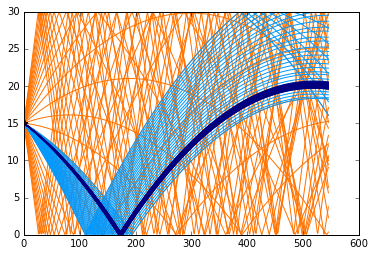
\includegraphics{ghia_sound_prop_curve}
  \caption{Non-Linear Marine Propagation in an isothermal profile}
  \todo[inline]{Vectorise and Label}
  \label{fig:ghia_sound_prop_curve}
\end{figure}


Comparing $A_{aco}(d,f)$ with the RF Free-Space Path Loss model $(A_{\text{RF}}(d,f) \approx \left( \frac{4\pi d f}{c} \right)^2)$, the impact of range on signal power is exponential underwater, rather than quadratic in terrestrial RF ($A_{\text{aco}} \propto f^{2d}$ vs $A_{\text{RF}} \propto (df)^2$). 
While both frequency dependant factors are quadratic, approximating the factors in \eqref{eq:thorp}, $f\propto A_{\text{aco}}$ is at least 4 orders of magnitude higher than $f\propto A_{\text{RF}}$

\subsection{Modelling and Simulation of the Acoustic Medium / Channel}

Several toolkits exist in a variety of states that perform communications agent simulation, most notably the NS-2 / 3 family of frameworks and their addons.
Some of these frameworks, such as SUNSET \cite{Petrioli2012a} and AquaTools \cite{Senghal2010}.

Beyond the NS family, there are many other communications and simulation modelling systems such as OpNet++\cite{Chang1999} and MATLAB toolkits such as the AcTUP interface to the Ocean Acoustics Library.


\todo{expand this, justify AUVNetSim, reactive mobility, python compatibility, SimPy Etc.}


\subsection{Routing and Network Design for \glspl{uan}}

Forward Error Correction coding is used on such channels to minimise packet losses.

\todo{Summary of Akyildiz02/05}

\subsection{Need for Trust in Maritime Networks}

As \acrfull{auv} platforms become more capable and economical, they are being used in many applications requiring trust.
These applications are using the collective behaviour of teams or fleets of these \glspl{auv} to accomplish tasks \cite{Caiti2011}.
With this use being increasingly isolated from stable communications networks, the establishment of trust between nodes is essential for the reliability and stability of such teams.
As such, the use of trust methods developed in the terrestrial \gls{manet} space must be re-appraised for application within the challenging underwater communications channel.

\todo{Possibly worth having some discussion on mobility in here}


\section{Grey System Theory and Grey Trust Assessment}
\todo{This section largely repeats from \acrshort{mtfm} discussion but the maths needs explored somewhere}
\subsection{Grey numbers, operators and terminology}
Grey numbers are used to represent values where their discrete value is unknown, where that number may take its possible value within an interval of potential values, generally written using the symbol $\oplus$.
Taking $a$ and $b$ as the lower and upper bounds of the grey interval respectively, such that $\oplus \in [a,b] | a < b$ 
The ``field'' of $\oplus$ is the value space $[a,b]$.
There are several classifications of grey numbers based on the relationships between these bounds.\todo{don't think classification is the right word here}
Black and White numbers are the extremes of this classification; such that $\dot\oplus \in [-\infty, +\infty]$ and $\mathring\oplus \in [x, x] | x \in \mathbb{R}$ or $\oplus(x)$
It is clear that white numbers such as $\mathring\oplus$ have a field of zero while black numbers have an infinite field.

Grey numbers may represent partial knowledge about a system or metric, and as such can represent half-open concepts, by only defining a single bound; for example $\underline\oplus = \oplus(\underline x ) \in [x, +\infty]$ and $\overline\oplus = \oplus(\overline x) \in [-\infty, x]$.

Primary operations within this number system are as follows;
\begin{subequations}
  \begin{align}
    \oplus_1 + \oplus_2      &\in [a_1+a_2,b_1+b_2] \label{eq:grey_add}\\
    -\oplus         &\in [-b,-a] \label{eq:grey_neg} \\
    \oplus_1 - \oplus_2      &= \oplus_1+(-\oplus) \label{eq:grey_sub}\\
    \oplus_1 \times \oplus_2 &\in \begin{aligned}[t]
      &[\min(a_1 a_2, a_1 b_2, b_1 a_2, b_2 a_2), \\
      & \max(a_1 a_2, a_1 b_2, b_1 a_2, b_2 a_2)]
    \end{aligned} \label{eq:grey_mult}\\
    \oplus^{-1} &\in [b^{-1}, a^{-1}] \label{eq:grey_inv}\\
    \oplus_1 / \oplus_2 & = \oplus_1 \times \oplus_2^{-1} \label{eq:grey_div} \\
    \oplus \times k &\in [ka,kb] \label{eq:grey_times_scalar}\\
    \oplus^k &\in [a^k, b^k] \label{eq:grey_exp}
  \end{align}
\end{subequations}
where $k$ is a scalar quantity.

\subsection{Whitenisation and the Grey Core}
The characterisation of grey numbers is based on the encapsulation of information in a grey system in terms of the grey numbers core ($\hat\oplus$) and it's degree of greyness ($g^\circ$).
If the distribution of a grey number field is unknown and continuous, $\hat\oplus = \frac{a + b}{2}$.

Non-essential grey numbers are those that can be represented by a white number obtained either through experience or particular method. \cite{Liu2011}
This white value is represented by $\tilde\oplus$ or $\oplus(x)$ to represent grey numbers with $x$ as their whitenisation.
In some cases depending on the context of application, particular gray numbers may temporarily have no reasonable whitenisation value (for instance, a black number).
Such numbers are said to be Essential grey numbers.

\subsection{Grey Sequence Buffers and Generators}
\todo{eqs of sequence buffers and partial derivs}
Given a fully populated value space, sequence buffer operations are used to provide abstractions over the dataspace.
These abstractions can be \emph{weakening} or \emph{strengthening}.
In the weakening case, these operations perform a level of smoothing on the volatility of a given input space, and strengthening buffers serve to highlight and 
A powerful tool in grey system theory is the use of grey incidence factors, comparing the ``likeness'' of one value against a cohort of values.
This usefulness applies particularly well in the case of multi-agent trust networks, where the aim is to detect and identify malicious or maladaptive behaviour, rather than an absolute assessment of ``trustworthiness''.

\subsection{Grey Trust}
Grey Theory performs cohort based normalization of metrics at runtime.
This creates a more stable contextual assessment of trust, providing a ``grade'' of trust compared to other observed entities in that interval, while maintaining the ability to reduce trust values to a stable assessment range for decision support without requiring every environment entered into to be characterised.
Grey assessments are relative in both fairly and unfairly operating cohorts.
Entities will receive mid-range trust assessments if there are no malicious actors as there is no-one else ``bad'' to compare against.

Guo\cite{Guo11} demonstrated the ability of Grey Relational Analysis (GRA)\cite{Zuo1995} to normalise and combine disparate traits of a communications link such as instantaneous throughput, received signal strength, etc.\ into a Grey Relational Coefficient, or a ``trust vector''.

In \cite{Guo11}, the observed metric set $X = {x_1,\dots,x_M}$ representing the measurements taken by each node of its neighbours at least interval, is defined as $X=[$packet loss rate, signal strength, data rate, delay, throughput$]$.
The trust vector is given as
%
\begin{align}
  \label{eq:grc}
  \theta_{k,j}^t = \frac{\min_k|a_{k,j}^t - g_j^t| + \rho \max_k|a_{k,j}^t-g_j^t|}{|a_{k,j}^t-g_j^t| + \rho \max_k|a_{k,j}^t-g_j^t|} \\
  \phi_{k,j}^t = \frac{\min_k|a_{k,j}^t - b_j^t| + \rho \max_k|a_{k,j}^t-b_j^t|}{|a_{k,j}^t-b_j^t| + \rho \max_k|a_{k,j}^t-b_j^t|} \notag 
\end{align}
%
where $a_{k,j}^t$ is the value of a observed metric $x_j$ for a given node $k$ at time $t$, $\rho$ is a distinguishing coefficient set to $0.5$, $g$ and $b$ are respectively the '``good'' and ``bad'' reference metric sequences from $\{a_{k,j}^t k=1,2\dots K\}$, e.g.\ $g_j=\max_k({a_{k,j}^t})$,  $b_j=\min_k({a_{k,j}^t})$ (where each metric is selected to be monotonically positive for trust assessment, e.g.\ higher throughput is always better).

Weighting can be applied before generating a scalar value which allows the identification and classification of untrustworthy behaviours.

%
\begin{equation}
  \label{eq:metric_weighting}
  [\theta_k^t, \phi_k^t] = \left[\sum_{j=0}^M h_j \theta_{k,j}^t,\sum_{j=0}^M h_j \phi_{k,j}^t \right]
\end{equation}
Where $H=[h_0\dots h_M]$ is a metric weighting vector such that $\sum h_j = 1$, and in the basic case, $H=[\frac{1}{M},\frac{1}{M}\dots\frac{1}{M}]$ to treat all metrics evenly.
$\theta$ and $\phi$ are then scaled to $[0,1]$ using the mapping $y = 1.5 x - 0.5$.
The $[\theta,\phi]$ values are reduced into a scalar trust value by $T_k^t = ({1+{(\phi_k^t)^2}/{(\theta_k^t)^2}})^{-1}$.
This trust value minimises the uncertainties of belonging to either best ($g$) or worst ($b$) sequences in \eqref{eq:grc}.

\acrshort{mtfm} combines this GRA with a topology-aware weighting scheme\eqref{eq:networkeffects} and a fuzzy whitenization model\eqref{eq:whitenization}.
There are three classes of topological trust relationship used; Direct, Recommendation, and Indirect.
Where an observing node, $n_i$, assesses the trust of another, target, node, $n_j$; the Direct relationship is $n_i$'s own observations $n_j$'s behaviour.
In the Recommendation case, a node $n_k$, which shares Direct relationships with both $n_i$ and $n_j$, gives its assessment of $n_j$ to $n_i$.
The Indirect case, similar to the Recommendation case, the recommender $n_k$, does not have a direct link with the observer $n_i$ but $n_k$ has a Direct link with the target node, $n_j$.
These relationships give us node sets, $N_R$ and $N_I$ containing the nodes that have recommendation or indirect, relationships to the observing node respectively.
%
\begin{align}
  \label{eq:networkeffects}
  T_{i,j}^{\acrshort{mtfm}}=\frac{1}{2} \cdot \max_s\{f_s(T_{i,j})\} T_{i,j}+&\frac{1}{2} \frac{2|N_R| }{2|N_R| + |N_I|}\sum_{n \in N_R} \max_s\{f_s(T_{i,n})\} T_{i,n}\\ \notag
  +&\frac{1}{2} \frac{|N_I| }{2|N_R| + |N_I|}\sum_{n \in N_I} \max_s\{f_s(T_{i,n})\} T_{i,n} 
\end{align}
Where $T_{i,n}$ is the subjective trust assessment of $n_i$ by $n_n$, and $f_s = [ f_1,f_2, f_3]$ given as:
\begin{align}
  \label{eq:whitenization}
  f_1(x)&= -x+1\notag\\
  f_2(x)&= 
  \begin{cases}
    2x & \text{if }x\leq 0.5\\
    -2x+2 & \text{if }x>0.5
  \end{cases}\\
  f_3(x)&= x\notag
\end{align}
Grey System Theory, by it's own authors admission, hasn't taken root in it's originally intended area of system modelling \cite{Liu2011}.
However, given it's tentative application to \gls{manet} trust, taking a Grey approach on a per metric benefit has qualitative benefits that require investigation; the algebraic approach to uncertainty and the application of ``essential and non essential greyness'', whiteisation, and particularly grey buffer sequencing allow for the opportunity to generate continuous trust assessments from multiple domains asynchronously.



%%%%%%%%%%%%%%%%%%%%%%%%%%%%%%%%%%%%%%%%%%%%%%%%%%%%%%%%%%%%%%%%%%%%%%%%%%%%%%%
\ifx\ifthesis\undefined
%% ----------------------------------------------------------------
\label{Bibliography}
% \bibliographystyle{amsplain}
%\bibliographystyle{unsrtnat}  % Use the "unsrtnat" BibTeX style for formatting the Bibliography
\bibliographystyle{alpha}
\bibliography{../Thesis}  % The references (bibliography) information are stored in the file named "Thesis.bib"

\end{document}  % The End
%% ----------------------------------------------------------------
\else
\fi

